\documentclass[border=10pt]{standalone}
\usepackage{fontspec}
\directlua{luaotfload.add_fallback("hmbfallback",{"Noto Serif CJK TC:mode=node;","Noto Serif CJK JP:mode=node;","Noto Serif CJK SC:mode=node;"})}
\setmainfont{Noto Serif}[RawFeature={fallback=hmbfallback}]
\setsansfont{Noto Sans}[RawFeature={fallback=hmbfallback}]
\setmonofont{Noto Sans Mono}[RawFeature={fallback=hmbfallback}]
\tracinglostchars=3
\directlua{
local hmblog = function(n, p) texio.write_nl("log", "HMB-SANDBOX-VIOLATION " .. n .. " " .. tostring(p)) end
local hmbin = function(p) return type(p) == "string" and (string.sub(p, 1, 5) == "/job/" or (not (string.sub(p, 1, 1) == "/") and not string.find(p, "..", 1, true))) end
local hmbblock = function(t, n) if t and t[n] then t[n] = function(...) hmblog(n, (...)); return nil, "blocked" end end end
local hmbpath = function(t, n) if t and t[n] then local f = t[n]; t[n] = function(p, ...) if not hmbin(p) then hmblog(n, p) end; return f(p, ...) end end end
hmbblock(os, "execute"); hmbblock(os, "exec"); hmbblock(os, "spawn"); hmbblock(io, "popen")
hmbpath(os, "remove"); hmbpath(os, "rename"); hmbpath(lfs, "mkdir"); hmbpath(lfs, "rmdir"); hmbpath(lfs, "touch"); hmbpath(lfs, "link"); hmbpath(lfs, "chdir")
local hmbopen = io.open
io.open = function(p, m, ...) if type(m) == "string" and string.find(m, "[wa+]") and not hmbin(p) then hmblog("io.open-write", p) end; return hmbopen(p, m, ...) end
}

\usepackage{tikz}
\usetikzlibrary{shapes.geometric, positioning, arrows.meta}

\begin{document}
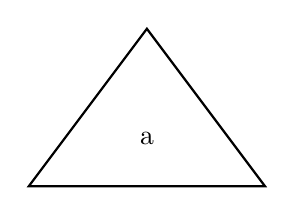
\begin{tikzpicture}
    % Define the vertices of the triangle. Let the base be horizontal.
    % We can place the triangle in a coordinate system.
    % Let the base be on the x-axis.
    % Let the apex be at the top.
    
    % Define coordinates for a general triangle shape.
    % For simplicity and to match the visual representation, we can use relative positioning or simple coordinates.
    
    % Let the base vertices be A and B, and the apex be C.
    % The image shows a triangle with a single label 'a' inside it.
    
    % We will define the triangle using coordinates.
    % Let the base be centered at (0, 0) for simplicity in placing 'a'.
    % Let the height be H and the base width be W.
    
    % To match the aspect ratio roughly, let's choose coordinates.
    % Let the base span from (-1.5, 0) to (1.5, 0).
    % Let the apex be at (0, 2).
    
    \coordinate (A) at (-1.5, 0);
    \coordinate (B) at (1.5, 0);
    \coordinate (C) at (0, 2);
    
    % Draw the triangle
    \draw[thick] (A) -- (B) -- (C) -- cycle;
    
    % Place the label 'a' inside the triangle.
    % The label 'a' is centered roughly in the lower half of the triangle.
    % We can estimate the center of the triangle or place it near the centroid/midpoint of the base.
    
    % Centroid calculation: ((x_A + x_B + x_C)/3, (y_A + y_B + y_C)/3)
    % Centroid = ((-1.5 + 1.5 + 0)/3, (0 + 0 + 2)/3) = (0, 2/3)
    
    % Place 'a' near the centroid.
    \node at (0, 0.6) {a};
    
\end{tikzpicture}
\end{document}
